\documentclass{standalone}
\usepackage{tikz}
\begin{document}
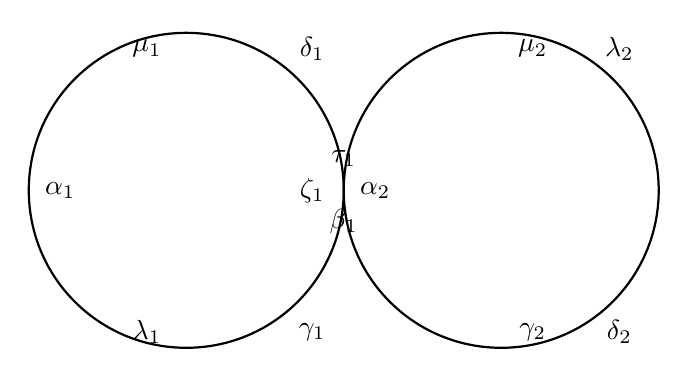
\begin{tikzpicture}
    % Left loop
    \draw[thick] (0,0) to[out=90, in=180] (2,2) 
        to[out=0, in=90] (4,0) 
        to[out=270, in=0] (2,-2) 
        to[out=180, in=270] (0,0);
    
    % Right loop
    \draw[thick] (4,0) to[out=270, in=180] (6,-2) 
        to[out=0, in=270] (8,0) 
        to[out=90, in=0] (6,2) 
        to[out=180, in=90] (4,0);
    
    % Labels for left loop
    \node at (0.4,0) {$\alpha_1$};
    \node at (1.5,1.8) {$\mu_1$};
    \node at (1.5,-1.8) {$\lambda_1$};
    \node at (3.6,1.8) {$\delta_1$};
    \node at (3.6,-1.8) {$\gamma_1$};
    
    % Labels for the connecting part
    \node at (4.4,0) {$\alpha_2$};
    \node at (4,0.4) {$\tau_1$};
    \node at (3.6,0) {$\zeta_1$};
    \node at (4,-0.4) {$\beta_1$};
    
    % Labels for right loop
    \node at (6.4,-1.8) {$\gamma_2$};
    \node at (6.4,1.8) {$\mu_2$};
    \node at (7.5,-1.8) {$\delta_2$};
    \node at (7.5,1.8) {$\lambda_2$};
    
\end{tikzpicture}
\end{document}